\documentclass{beamer}
\usepackage{pgfpages}
%\setbeameroption{show notes on second screen=left} %enable for notes
\usepackage{graphicx}
\usepackage{xcolor}
\usepackage{listings}
%\usepackage{transparent}
\usepackage{hyperref}
\lstset{language=python,frame=single}
\usepackage{verbatim}
%\usepackage{apacite}
\usepackage[longnamesfirst]{natbib}
\usepackage{subcaption}
\usepackage{amsmath}
\usepackage{relsize}
\usepackage{appendixnumberbeamer}
\usepackage{xparse}
\usepackage{multimedia}
\usepackage{xcolor}
\usepackage[normalem]{ulem}
\usepackage{tikz}
\usetikzlibrary{matrix,backgrounds}
\usetikzlibrary{positioning}
\usetikzlibrary{shapes,arrows}
\usetikzlibrary{positioning}

\tikzset{onslide/.code args={<#1>#2}{%
  \only<#1>{\pgfkeysalso{#2}} 
}}

\tikzstyle{block} = [rectangle, draw, fill=red!20!blue!10, 
    text width=5em, text centered, rounded corners, minimum height=4em]
\tikzstyle{netnode} = [circle, draw, very thick, inner sep=0pt, minimum size=0.5cm] 
\tikzstyle{relunode} = [rectangle, draw, very thick, inner sep=0pt, minimum size=0.5cm] 
    
\tikzstyle{line} = [draw, line width=1.5pt, -latex']

\pgfdeclarelayer{background}
\pgfsetlayers{background,main}

\pgfdeclarelayer{myback}
\pgfsetlayers{myback,background,main}

\usetheme[numbering=fraction]{metropolis}

\newcommand\blfootnote[1]{%
  \begingroup
  \renewcommand\thefootnote{}\footnote{#1}%
  \addtocounter{footnote}{-1}%
  \endgroup
}
\renewcommand*\footnoterule{}
%%\AtBeginSection[]
%%{
%%  \begin{frame}
%%    \frametitle{Table of Contents}
%%    \tableofcontents[currentsection]
%%  \end{frame}
%%}

\begin{document}

\title{}
\author{Andrew Lampinen}
\date{FriSem, 5/11/2018}
\frame{\titlepage}

\begin{frame}[standout]
How do people learn so rapidly? \par
\only<2->{Claim: Transfer.}
\end{frame}


\begin{frame}{Transfer across domains}
Not a new idea: e.g. \cite{Gick1980, Gentner2003}
\uncover<2>{
\only<-2>{
\begin{figure}
\centering
\begin{subfigure}{0.4\textwidth}
\includegraphics[width=\textwidth]{figures/chess_cropped.jpg}
\end{subfigure}%
\begin{subfigure}{0.4\textwidth}
\includegraphics[width=\textwidth]{figures/go.jpg}
\end{subfigure}\\
\begin{subfigure}{0.4\textwidth}
\includegraphics[width=\textwidth]{figures/math.jpg}
\end{subfigure}%
\begin{subfigure}{0.4\textwidth}
\includegraphics[width=\textwidth]{figures/piano.jpg}
\end{subfigure}%
\end{figure}
}
}
\only<3>{
\begin{figure}
\centering
\includegraphics[width=0.8\textwidth]{figures/category_theory.jpg}
\end{figure}
}
\uncover<2->{
\scriptsize
\citep{Lampinen2017, Hansen2017}
}
\note{There are deep relationships among the tasks we do -- some are superficially obvious, like Go and Chess, and some are less so, like the mathematical structures underlying music or the fact that we use language to talk about all these domains.\par
Of particular interest to me is deep isomorphisms between mathematical domains, and this is actually one of the things that inspired Gick \& Holyoak.}
\end{frame}

\begin{frame}{Criticism?}
However, this perspective has been criticized!\par
\begin{itemize}
\item<2-> ``Significant transfer is probably rare and accounts for very little human behavior.'' \citep{Detterman1993}
\item<3-> From FriSem last year: 
\begin{figure}
\centering
\includegraphics[width=0.4\textwidth]{figures/perspectives_on_transfer.png}
\end{figure}
\end{itemize}
\note{Detterman: ``We generally do what we have learned to do and no more.'' Experimental manipulations in transfer experiments ``have the subtlety of a baseball bat.''\par
Observation from FriSem last year: there is a correlation between the speed of transfer being sought and how important they think it is.}
\end{frame}

\begin{frame}{Transfer speed}
\vspace{1.5em}
What do I mean by ``fast'' and ``slow?''\par
\uncover<2->{
\begin{center}
\begin{table}
\begin{tabular}{|c|c|}
\hline
Fast & Slow \\
\hline
\parbox{0.45\textwidth}{
    \begin{itemize}
    \item<2-> one (or a few) examples explicitly shown
    \item<3-> transfer requires explicit awareness of analogy\\[5em]
    \end{itemize}
}
&
\parbox{0.45\textwidth}{
    \begin{itemize}
    \item<2-> learning through many interactions
    \item<3-> {transfer may or may not be explicit}%
               %%\only<4>{\color{red}transfer may or may not be explicit}}
    \item<4-> may take developmental time, or at least a long experiment!
    \end{itemize}
}\\ \hline
\end{tabular}
\end{table}
}
\vspace{1.5em}
\note{E.g. being told about the rules of chess and then seeing if that helps you play go, vs. playing many games of chess and go and seeing if one helps the other}
\end{center}
{
\scriptsize
\citep{Lampinen2017}
}
\end{frame}

\begin{frame}[standout]
Slow transfer between tasks is important.
\end{frame}

\begin{frame}{Abstraction as a kind of transfer}
We often progress from procedural to more formal knowledge, e.g. in mathematics:
\begin{figure}
\centering
\begin{tikzpicture}
\node (img1) {\includegraphics[width=0.33\textwidth]{figures/multiplication_procedural_smaller.png}};
\only<2->{
\node (img2) at ([yshift=-2em]img1.east) {\includegraphics[width=0.33\textwidth]{figures/factoring_polynomial_worksheet.png}};
}
\only<3->{
\node (img3) at ([yshift=-3em]img2.east) {\includegraphics[width=0.5\textwidth]{figures/prime_ideals.png}};
}
\end{tikzpicture}
\end{figure}
\uncover<4>{This can be seen as a kind of transfer!}
\note{worksheetfun.com\par
Less abstract and more abstract reasoning can be seen as partially distinct tasks that share some common structure. There are different ways that procedural knowledge could support more formal, setting up representations and intuitions, having examples to reason over, ...}
\end{frame}

\begin{frame}[standout]
Abstraction is one type of task where we might look for transfer.
\end{frame}

\begin{frame}{A diagram of potential phenomena of interest}
\begin{figure}
\centering
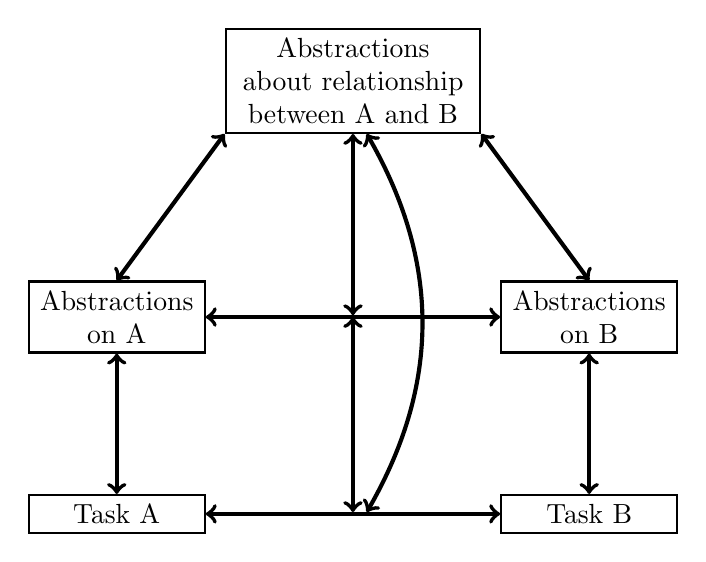
\begin{tikzpicture}[auto] %% TODO? highlighting
\node [rectangle, draw, thick, text width=2cm, align=center ] (A) at (-3, 0) {Task A}; 
\node [rectangle, draw, thick, text width=2cm, align=center] (B) at (3, 0) {Task B}; 
\uncover<2->{
\path [line, <->] (A.east) to node (proctrans) {} (B.west); 
}
\uncover<3->{
\node [rectangle, draw, thick, text width=2cm, align=center] (Aabs) at (-3, 2.5) {Abstractions on A}; 
\node [rectangle, draw, thick, text width=2cm, align=center] (Babs) at (3, 2.5) {Abstractions on B}; 
\path [line, <->] (A.north) to  node (Atrans) {}(Aabs.south); 
\path [line, <->] (B.north) to node (Btrans) {} (Babs.south); 
}
\uncover<4->{
\path [line, <->] (Aabs.east) to node (abstrans) {} (Babs.west); 
}
\uncover<5->{
\path [line, <->] ([yshift=-0.75em]proctrans.north) to node (procabstrans) {} (abstrans.south); 
}
\uncover<6->{
\node [rectangle, draw, thick, text width=3cm, align=center] (ABabs) at (0, 5.5) {Abstractions about relationship between A and B}; 
}
\uncover<7->{
\path [line, <->] (Aabs.north) to  (ABabs.south west); 
\path [line, <->] (Babs.north) to  (ABabs.south east); 
}
\uncover<8->{
\path [line, <->] ([yshift=-0.75em]abstrans.north) to(ABabs.south); 
\path [line, <->, bend right] ([xshift=0.5em, yshift=-0.75em]proctrans.north) to([xshift=0.5em]ABabs.south); 
}

\end{tikzpicture}
\end{figure}

\end{frame}

\section{Experimental design}

\begin{frame}[allowframebreaks]
\bibliographystyle{plainnat}
\blfootnote{\bibliography{transfer}}
\end{frame}
\end{document}
